\documentclass{beamer}
\usetheme{Frankfurt}
\usepackage{graphicx}
\usepackage{amsmath}
\title{Quyoshni kuzatish tizimiga ega fotoelektrik issiqlik qurilmalarining parametrlarini asoslash}
\subtitle{}
\author{Jumayev Tursunboy Xusen o`g`li}
\institute{\texttt Mutaxassislik: 5A140204 -- Fizika (yo`nalishlar bo`yicha). Lazer fizikasi}
\date{\today}

\begin{document}
\begin{frame}
	\titlepage
\end{frame}

\begin{frame}
	\renewcommand{\contentsname}{Mundarija}
	\tableofcontents
\end{frame}
\begin{frame}{Kirish}
	\section{Kirish}
	Kvant fizikasining asoschilaridan biri M. Plank 1879-yili Myunxenda dissertatsiyasini himoya qilgandan keyin ustozi Filip fon-Jolliga nazariy fizika bilan shug`ullanish niyati borligini aytadi. Ustoz esa o`z navbatida nazariy fizika poyoniga yetgani, faqat ba'zi xususiy hollar, boshlang`ich va chegaraviy shartlarni o`zgartirib differensial tenglamalarning yechimini topish qolgani, umuman, bu "istiqbolsiz ish" bilan shug`ullanish befoydaligini uqtiradi.
\end{frame}
\begin{frame}{Kirish}
	Shunga qaramay, Plank nazariy fizika bilan shug`ullanishni davom ettirib, 1900-yili elektromagnit nurlanishning diskret ekanligini kashf qildi. 1905-yilda Eynshteyn tomonidan elektromagnit maydonning energiyasi diskret strukturaga egaligi, undagi eng kichik zarra fotonni aniqlaydi, keyinchalik atomning kvant nazariyasi va kvant mexanikaga asos soladi. U davrda kvant mexanikasi tushunchalarining ilm ahli tomonidan qabul qilinishi juda qiyin kechdi. Boisi, birinchidan, kichik zarralarning kichik o`lchamlarda harakat traektoriyasi degan tushunchaning yo`qligi, ikkinchidan, Veyner Geyzenberg tomonidan kiritilgan noaniqlik prinsipi edi. Unga ko`ra, kichik o`lchamlarda zarrachaning impulsi va koordinatasi (energiya yoki vaqt)ni bir vaqtda katta aniqlikda o`lchab bo`lmaydi.
\end{frame}
\begin{frame}{Fotoelementlar}
	\section{Fotoelementlar}
	Fotoelement (\textit{photo} va \textit{element}) -- o`ziga tushayotgan yorug`likni yutib, elektr toki (fototok) yoki foto elektr yurituvchi kuch hosil qiluvchi elektr asbob. Ishlash prinsipi fotoelektron emissiya yoki ichki fotoeffekt hodisasiga asoslangan. Fotoelektron emissiya asosida ishlaydigan fotoelement vakuum hosil qilingan yoki gaz to`ldirilgan shisha, yoxud kvars kolba ichiga joylangan ikki elektrod - fotokatod va anodli elektrovakuum asbobdan iborat. Fotokatodga tushadigan yorug`lik oqimi uning sirtida fotoelektron emissiya hosil qiladi; Fotoelement zanjiri tutashtirilganda unda yorug`lik oqimiga monand fototok oqimi vujudga keladi. 
\end{frame}

\begin{frame}
	\begin{columns}[T]
		\begin{column}{.5\textwidth}
			\begin{block}{Fotoelement}
				Gaz to`ldirilgan fotoelementda gazning ionlanishi va nomustaqil kuchli razryad hosil bo`lishi natijasida fototok kuchayadi. Ichki fotoeffekt asosida ishlaydigan fotoelementlarda gomogen elektron-kovak o`tish (n-p o`tish), yarimo`tkazgich, geteroo`tishli yoki metall-yarimo`tkazgich kontaktli yarimo`tkazgich asbobdan iborat. Bunday fotoelementda optik nurlar yutilib, zaryad tashuvchilar konsentratsiyasi ortadi va elektr yurituvchi kuch hosil bo`ladi. 
			\end{block}
		\end{column}
		\begin{column}{.5\textwidth}
			\begin{block}{rasm1}
				\begin{figure*}
					\centering
					\begin{figure*}
						\centering
						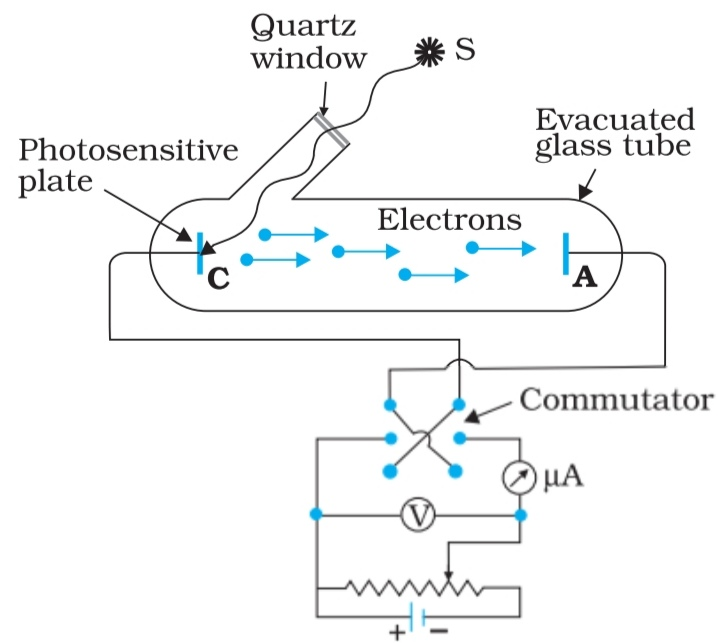
\includegraphics[width=0.7\linewidth]{9kd2f}
						\caption{}
						\label{fig:9kd2f}
					\end{figure*}
				\end{figure*}
			\end{block}
		\end{column}
	\end{columns}
\end{frame}


\begin{frame}
	
	 \begin{columns}[T]
		\begin{column}{.25\textwidth}
			\begin{block}{}
rasm 2
			\end{block}
		\end{column}
		\begin{column}{.75\textwidth}
			\begin{block}{}
				\begin{figure*}
					\centering
					\begin{figure*}
						\centering
						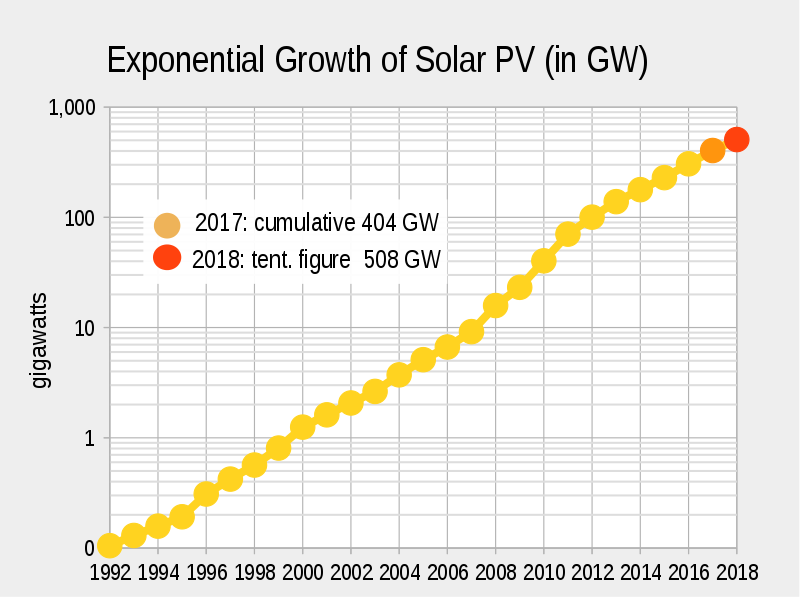
\includegraphics[width=0.7\linewidth]{800px-PV_cume_semi_log_chart_2014_estimate.svg}
						\caption{}
						\label{fig:800px-pvcumesemilogchart2014estimate}
					\end{figure*}
				\end{figure*}
			\end{block}
		\end{column}
	\end{columns}
\end{frame}

\begin{frame}{}
	    \Huge{E'tiboringiz uchun rahmat!}
\end{frame}

\end{document}
